\documentclass{article}

\usepackage[utf8]{inputenc}
\usepackage[T1]{fontenc}
\usepackage[portuguese]{babel}

\usepackage{amsmath}
\usepackage{graphicx}
\usepackage{float}
\usepackage{subcaption}
\usepackage[colorlinks=true]{hyperref}


\title{Projeto final processo seletivo Equipe Phoneix 2017}
\author{
    Integrantes:\\
    Carlos Henrique Coelho Miyazawa\\
    Guilherme Birta de Souza\\
    Luiz Eduardo Araujo Zucchi\\
    Marco Antonio Steck Filho\\
    Vitor Hugo Nascimento Silva\\
    \\
    Monitora: Luísa Starling
}
\date{\today}

\begin{document}
    \maketitle
    \newpage
    \tableofcontents
    \newpage

    \section{Resumo}
        \subsection{Descrição}
        \paragraph{}
        O robô aqui descrito é um robô da categoria Hobbyweight que consiste de uma categoria de robôs de luta que pesam até 12libras(cerca de 5,5kg) controlados por rádio e, no nosso caso, utilizando um controle de PlayStation2(DualShock2), tal robô deverá tentar infligir danos no robô adversário utilizando-se de uma arma arbitrariamente escolhida.

        \subsection{Estrutura}
        \paragraph{}
        O robô projetado por nossa equipe é constituído por uma lâmina giratória posicionada em sua frente(sua arma) e
        sua carcaça será triangular com apenas duas rodas de diametro maior que sua altura, possibilitando um fácil
        controle não importando o lado no qual o robô está virado. O robô teria $30cm$ de largura, $40cm$ de
        comprimento(ponta a ponta) e sua altura 10cm.

        \begin{figure}[H]
        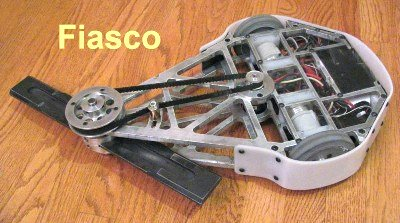
\includegraphics[width=\textwidth]{images/image05.jpg}
        \caption{Robô \textit{"fiasco"} no qual o nosso se baseia.}
        \centering
        \end{figure}

        \subsection{Projeto}
        \paragraph{}
        O projeto foi desenvolvido ao longo de 2 encontros de aproximadamente 1:30h cada, durante estas sessões o grupo
        decidiu em conjunto que curso tomariamos no desenveolvimento deste robô, ao final de cada encontro definimos
        metas para cada departamento cumprir, ou seja, ao final de cada encontro todos os membros saíram com um
        objetivo para sua parte do projeto. A ata da segunda reunião, com todos os membros presentes pode ser
        encontrada em: https://github.com/steckmarco/ps-phoenix/

    \section{Atividades departamentais}
        \subsection{Mecânica}
            \subsubsection{Rodas}
                \paragraph{}
                Podemos utilizar 2 rodas de borracha vulcanizadas, pois são muito resistentes, irão tornar o robô ágil, preço acessível e possível encomenda com as dimensões necessárias, que, nesse caso, deverão ser 50mm com raio de 5cm, para que quando o robô virar, não haver alterações na forma de locomoção.
                \\
                Valor: $R\$136,59$
            \subsubsection{Armadura}
                \paragraph{}
                A armadura será composta por alumínio aeronáutico 6,35mm, uma vez que esse não amassa facilmente, é muito resistente e absorve bem os impactos.
                Área total da armadura: 2600 $cm^2$
                \\
                Valor: $R\$238,97$
            \subsubsection{Arma}
                \paragraph{}
                A arma será uma hélice de impacto composta por aço SAE 4340, com dimensões de 8 cm de comprimento por 2,5cm de largura e 2cm de espessura.
                \\
                Peso: 314g\\
                Preço: $R\$85,00$


        \subsection{Elétrica e eletrônica}
            \subsubsection{Placa Controladora}
                \paragraph{}
                Na parte eletrônica de locomoção será usado uma placa Scorpion XL, pois ela é apropriada a robôs de combate, e nela consiste em uma ponte H onde se pode fazer a inversão dos motores sem ser necessária a criação de tensões negativas ou desconectar os terminais para que eles sejam trocados. Iremos utilizar o seu BEC interno, para diminuir a tensão de entrada, e também por ter uma bateria de tensão de entrada não muito alta que necessite de um BEC externo, o qual pode ser desativado se necessário. O controle de giro pode ser opcionalmente conectado através de um canal R/C ou por um interruptor mecânico (gravidade) ou óptico, caso o robô fique invertido.

                \begin{figure}[H]
                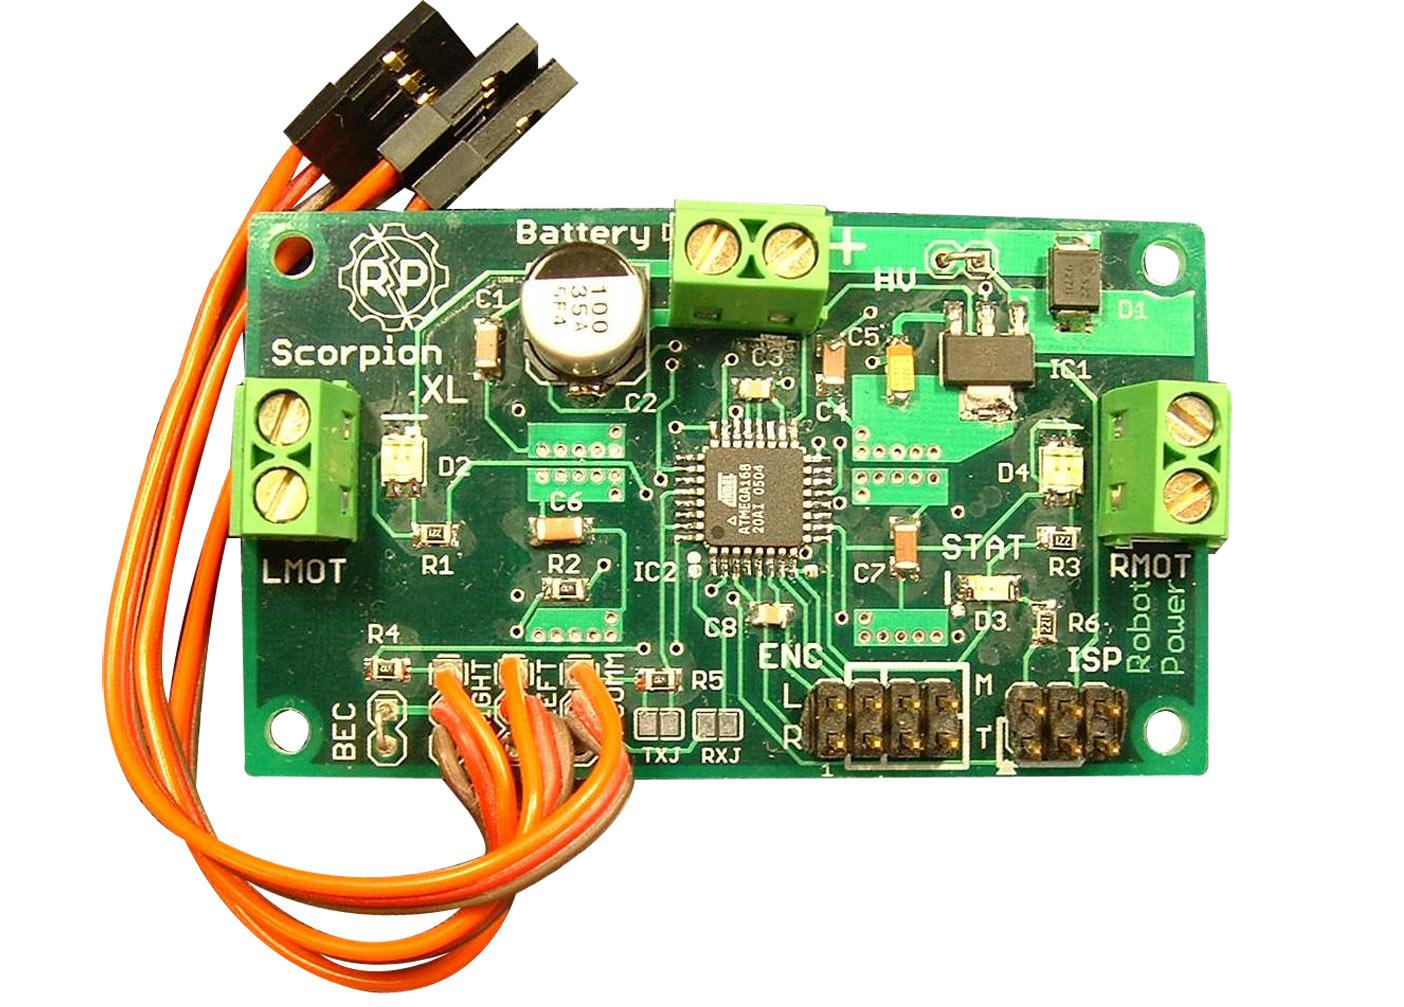
\includegraphics[width=\textwidth]{images/image00.jpg}
                \caption{Placa Scorpion XL}
                \centering
                \end{figure}

                \textbf{Especificações placa Scorpion:}
                \begin{itemize}
                    \item Tamanho: 68,58 x 40,64 x 12,7 mm
                    \item Peso: 28 gramas
                    \item três cabos de entrada R / C para
                    \item Unidade esquerda e direita - totalmente reversível H
                    \item Tensão da bateria de 4.8V a 28V
                    \item Corrente contínua de 12,5 A (pico de 45 A) em cada canal de accionamento esquerdo e direito. Pode ser combinado num único canal de avanço / retrocesso contínuo de 25 A. Esta é uma classificação 12.5A real, ou seja, você pode colocar 12.5A através dos canais de saída para severalminutes com picos mais altos por alguns segundos
                    \item Circuito eliminador de bateria do receptor (BEC) padrão - pode ser desabilitado.
                    \item Função de calibração para corresponder ao Scorpion ao seu rádio ou a outras fontes de sinal - configurações armazenadas na EEPROM
                    \item Preço: $R\$ 309,02$
                \end{itemize}

            \subsubsection{Bateria}
                \paragraph{}
                A bateria que será utilizada é do tipo LiPO Turnigy 5S de capacidade 4000 mAh, o que era suficiente para manter o robô funcionando com excelente performance durante o round inteiro. Essa bateria foi escolhida devido sua fácil recarga, tanto no quesito de tempo, quanto na eficiência de recarga, além de suprir as necessidades energéticas do sistema.
                \paragraph{}
                Como essas baterias (do tipo LiPO) são altamente explosivas, bem como perigosas no seu manuseio e uso, isolaremos os conectores das células da bateria a fim de que não haja curto circuitos.

                \begin{figure}[H]
                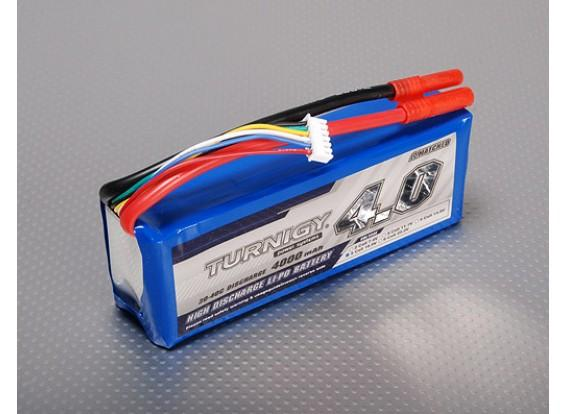
\includegraphics[width=\textwidth]{images/image02.jpg}
                \caption{Bateria LiPo}
                \centering
                \end{figure}

                \textbf{Especificações bateria Turnigy:}
                \begin{itemize}
                    \item Tamanho: 148 x 49 x 33 mm
                    \item Peso: 536g
                    \item Capacidade mínima: 5000mAh
                    \item Configuração: 5S1P / 18.5v / 5Cell
                    \item Descarga Constante: 30C
                    \item Pico de descarga (10sec): 40C
                    \item Preço: $R\$ 114.20$
                \end{itemize}

            \subsubsection{Motor de locomoção}
                \paragraph{}
                Para a locomoção, serão utilizados dois motores da marca polulu. Estes moto-redutores consistem em motores do tipo DC de 12V escovados de baixa potência, combinado com uma caixa de engrenagens de metal de 34 :1. Estes motores serão submetidos à tensão de saída da bateria, o qual é de 18,5V, pois a tensão utilizada é maior do que o normal e terem sido fabricados para o uso de 12V. Assim, o robô terá uma excelente performance durante o tempo do round sem prejudicar a constituição interna do motor.
                \paragraph{}
                Como o motor será submetido sob essa modificação, as especificações nominais serão alteradas de forma com que o eixo principal rodará com frequência maior do que 150 RPM, corrente de 100 mA, torque acima de 3 kgf.cm.

                \begin{figure}[H]
                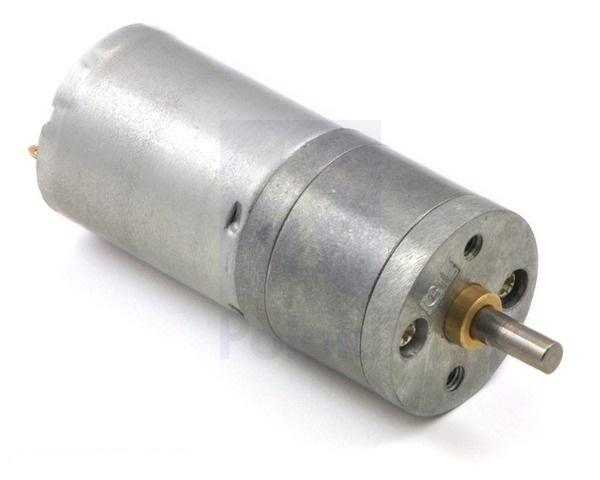
\includegraphics[width=\textwidth]{images/image01.jpg}
                \caption{Motor de locomoção}
                \centering
                \end{figure}

                \textbf{Especificações bateria Turnigy:}
                \begin{itemize}
                    \item Tensão: 12V
                    \item Velocidade de funcionamento livre 12V: 150 rpm
                    \item Torque: 3 kgf.cm
                    \item Peso: 88g
                    \item Diâmetro do eixo: 4 mm
                    \item Tamanho: 25D x 52L mm
                    \item Corrente livre: 100 mA
                    \item Corrente máxima: 1100 mA
                    \item Relação de engrenagem: 34,014: 1
                    \item Preço: $R\$ 61,69$
                \end{itemize}

            \subsubsection{Motor da arma}
                \paragraph{}
                Para a arma do tipo Spinner, acreditamos ser mais eficiente a utilização do motor Turnigy L3010B-1300 Brushless Motor (420w), porque ele atende a maioria das necessidades básicas de um robô spinner, uma vez que possui um Kv de 1300 RPM/V, já que a tensão aplicada nele será também de 18,5V, o que supera sua tensão nominal em 6,4V. Ainda que a tensão aplicada é maior, não há comprometimento com o funcionamento do motor para um tempo de combate pequeno. Essa técnica é muito utilizada nas competições de combate e geram ótimos resultados para a equipe.
                \paragraph{}
                Na eletrônica da arma utilizamos a placa controladora de motores brushless (BESC) Turnigy AE-100A, porque ela auxilia na eficiência do motor, a qual tem um microprocessador de alta performance compatível com vários tipos de motores, além disso, possui uma suave, linear, rápida e precisa resposta da aceleração, bem como contém proteção de alto aquecimento, sobrecarga, curto circuito, baixa voltagem e perda de aceleração do processo.

                \begin{figure}[H]
                \centering
                \begin{subfigure}[b]{0.75\textwidth}
                    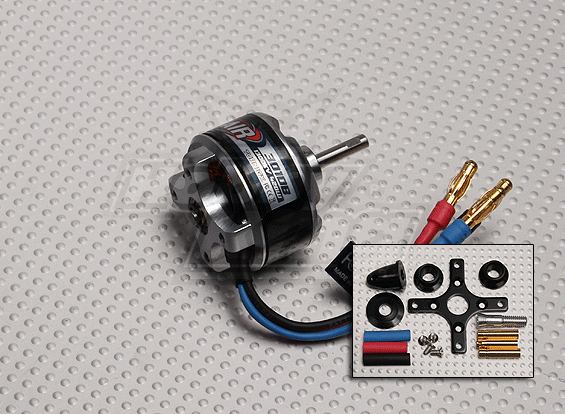
\includegraphics[width=\textwidth]{images/image04.jpg}
                    \caption{Motor da arma}
                \end{subfigure}
                \begin{subfigure}[b]{0.75\textwidth}
                    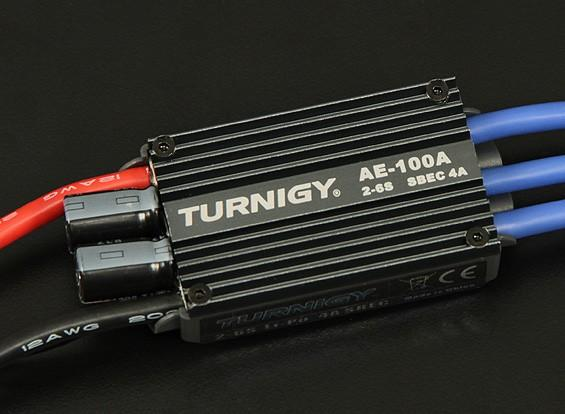
\includegraphics[width=\textwidth]{images/image03.jpg}
                    \caption{Placa controladora do motor}
                \end{subfigure}
                \end{figure}

                \textbf{Especificações do motor da arma:}
                \begin{itemize}
                    \item Tamanho: 37 x 27mm
                    \item Peso: 88g (108g com todos os acessórios, conectores e motorista de suporte)
                    \item Kv: 1300 rpm / V
                    \item Voltagem: 11,1v (3s)
                    \item Potência máxima: 420w
                    \item Corrente máx: 40.1A
                    \item Sem carga Corrente: 1.8A
                    \item Diâmetro do eixo: 4mm
                    \item Preço: $R\$ 51,64$
                \end{itemize}

                \textbf{Especificações da placa eletrônica do motor da arma:}
                \begin{itemize}
                    \item Saída: Contínuo 100A, explosão 115A até 10 segundos.
                    \item Tensão da entrada: 2-6 células de bateria de lítio ou 5-18 células NIMH bateria.
                    \item BEC: Linear 4A @ 5V
                    \item Sinal de Controle Transmissão: Sistema acoplado opticamente.
                    \item 2 Polo: 210.000 rpm
                    \item 6 Polo: 70.000 rpm
                    \item Polo 12: 35.000 rpm
                    \item Tamanho: 71 x 34 x 17mm.
                    \item Peso: 79g.
                    \item Preço: $R\$ 147,07$
                \end{itemize}

            \subsubsection{Preço final}
                \paragraph{}
                Somando-se os preços encontrados para cada peça aqui citada temos o preço total de $R\$ 745,49$ para a parte de elétrica e eletrônica. No apêndice estão listado os links para os sites de compra para estas peças.

        \subsection{Computação}
            \subsubsection{Placa externa}
                \paragraph{Algoritmo}
                \label{sec:1}
                \subparagraph{}
                O algorítimo de comunicação da placa externa com a interna se comportará do seguinte modo:
                \begin{enumerate}
                    \item Inicializa todas as funções de baixo nível.
                    \item Estabelece conexão com o controle na placa externa.
                    \item Loop infinito:
                    \begin{enumerate}
                        \item Ler dados do controle e identificar os botões relevantes pressionados.
                        \item Se for botão analógico mapear a intensidade para a variável $\textit{intesity}$ o valor entre 0 e 255 e para a variavel \textit{sinal}(que indica o sinal antes do mapeamento).
                        \item Transcrever os botões pressionados para os comandos estabelecidos na tabela \ref{tab:1}.
                        \item Transmitir os comandos para a placa interna do robô via sinal de rádio de 2.4GHz por meio do comando enviaDados(int Size, char byte...).
                    \end{enumerate}
                \end{enumerate}
                \textit{*Note que devemos ter também um circuito de watchdog para caso a execução congele a placa seja reiniciada automaticamente.}

                \paragraph{}
                Os dados são enviados na ordem que aparecem na figura \ref{tab:1} e são todos enviados ao mesmo tempo, ou seja, o size passado para a função é 7.
                \begin{table}[H]
                    \centering
                    \caption{Mapeamento dos botões pressionados para os comandos do robô.}
                    \label{tab:1}
                    \begin{tabular}{|l|l|l|}
                    \hline
                    Botão              & Comando                                  & Chars  enviados             \\ \hline
                    Analógico esquerdo & Controla potência do movimento           & {[}intensity, sinal{]}          \\
                    Analógico direito  & Controle de direção                      & {[}intensity, sinal{]}          \\
                    Botão X            & Altenar estado da arma(ligado/desligado) & {[}pressed{]}                   \\
                    Botão R2           & Acelerar                                 & {[}pressed{]}                   \\
                    Botão L2           & Reverso                                  & {[}pressed{]}                   \\ \hline
                    \end{tabular}
                \end{table}
                \textit{*Assume-se que as funções enviaDados da placa externa e a scanDados da placa interna garantem a integridade da mensagem por elas trocadas e sua ordem de chegada.}

                \paragraph{Ajustes dos analógicos}
                \subparagraph{}
                Além do algorítimo descrito na seção \ref{sec:1} o software da placa externa deverá apresentar alguns ajustes, como a definição de uma \textit{"deadzone"} para o controle, ou seja, a definição de um nível de sensibilidade dos analógicos no qual a placa deve ignorar o que está recebendo, isso se deve à possibilidade de a posição de descanso destes analógicos não estar corretamente centralizada e, portanto, essa \textit{"deadzone"} promoverá um controle mais preciso sobre as ações do robô.

            \subsubsection{Placa Interna}
                \paragraph{Algoritmo}
                \begin{enumerate}
                    \item Chamar a função configuraPerifericosPlacaInterna(), para que ela seja configurado.
                    \item Criar um loop que será mantido enquanto o robo permanecer ligado
                    \begin{enumerate}
                        \item Checar se ainda há conexão com a placa externa
                        \begin{enumerate}
                            \item Se não houver, tentar reestabelecer, ou reiniciar, caso falhe.
                            \item Através de um wacthdog, checar se a função não travou, se travar, reiniciar.
                            \item Se houver, continuar.
                        \end{enumerate}
                        \item Ler o número de comandos que devem ser recebidos, lendo apenas um byte.
                        \item Guardar os comandos reccebidos em um ponteiro relativo, depois, guardar esses ponteiros numa fila , na ordem q eles chegaram,
                        \item Processar os membors da fila, até chegar ao seu final, a cada membro processado, esperar receber retorno de sucesso do componente comandado (motor por exemplo), caso negativo tentar reenviar, após certo numero de tentativas, voltar ao começo do for para tentar reestabelecer conexão com a placa
                    \end{enumerate}
                \end{enumerate}

                \paragraph{Justificativa}
                \subparagraph{}
                A escolha de uma fila para guardar os bits, se justifica pelo fato de filas serem estruturas de dados, que de forma nativa seguem o principio FIFO (first-in, first-out). Após cada processo o recebimento de um retorno confirmando que a ação foi executada, é importante pois, dessa forma, um mal contato causado por imapctos, pode ser contornado, aumentando assim a duração do robo em combate.

\begin{appendix}
    \section{Peças da elétrica}
    \subsection{Controlador de velocidade}
    \begin{itemize}
        \item \url{http://www.robotmarketplace.com/products/0-scorp-xl.html}
        \item \url{http://www.robotcombat.com/products/images/0-SCORP-XL_quickstart.pdf}
        \item \url{http://financeone.com.br/moedas/conversor-de-moedas }
    \end{itemize}
    \subsection{Bateria}
    \begin{itemize}
        \item \url{https://hobbyking.com/en_us/turnigy-4000mah-5s-30c-lipo-pack.html }
    \end{itemize}
    \subsection{Motor de locomoção}
    \begin{itemize}
        \item \url{https://www.pololu.com/product/3252/specs}
    \end{itemize}
    \subsection{Motor da arma}
    \begin{itemize}
        \item \url{https://hobbyking.com/en_us/turnigy-l3010b-1300-brushless-motor-420w.html?gclid=CjwKEAjwq5LHBRCN0YLf9-GyywYSJAAhOw6maTrrm9zLg6r3b1X1Qqro43pdpV_i0s4LgRj9A4g1IBoCFJ_w_wcB&gclsrc=aw.ds}
    \end{itemize}
    \subsection{Placa Eletrônica do motor da arma}
    \begin{itemize}
        \item \url{https://hobbyking.com/en_us/turnigy-ae-100a-brushless-esc.html}
        \item \url{https://hobbyking.com/media/file/1038005134X342477X5.jpg}
    \end{itemize}

    \section{Outras fontes}
    \begin{itemize}
        \item \url{http://www.robot.bmstu.ru/files/books/[Robotic]%20Tutorial%20RioBotz.pdf}
        \item \url{http://financeone.com.br/moedas/conversor-de-moedas}
        \item \url{http://www.amazon.com}
        \item \url{https://www.robocore.net/modules.php?name=GR_LojaVirtual}
        \item \url{http://www.robotmarketplace.com/}
        \item \url{http://riobotz.com/pb/tutorials/}
    \end{itemize}

\end{appendix}
\end{document}
